A compensation for the image plane rotation of a face can be achieved by taking advantage of the symmetry of faces, namely that both eyes most often form a vector that is parallel to the horizontal axis. After the extraction of such a vector, one can easily find the rotation of the face.

The algorithm we use to locate the eyes is called the \textit{Circular Hough Transform} (CHT) which is a feature extraction technique for finding circles. The algorithm is popular and often used because of its robustness in noisy areas and tolerance for occlusion and varying illumination \cite{cht}. However, it does not exists a specific definition of the algorithm steps based on CHT. A brief description of a customized version is included below.

% https://www.cis.rit.edu/class/simg782/lectures/lecture_10/lec782_05_10.pdf

% http://docs.opencv.org/2.4/doc/tutorials/imgproc/imgtrans/hough_circle/hough_circle.html

The first step is to locate pixels at regions with high gradient variations. These pixels are called candidate pixels and they have the ability to cast \textit{votes}, in a circular pattern around themselves. An accumulator array is then defined to store the votes. More votes on a pixel increases the likelihood of it being a center point for a circle. The vote-pattern is illustrated by Figure \ref{fig:CHT}.

\begin{figure}[H]
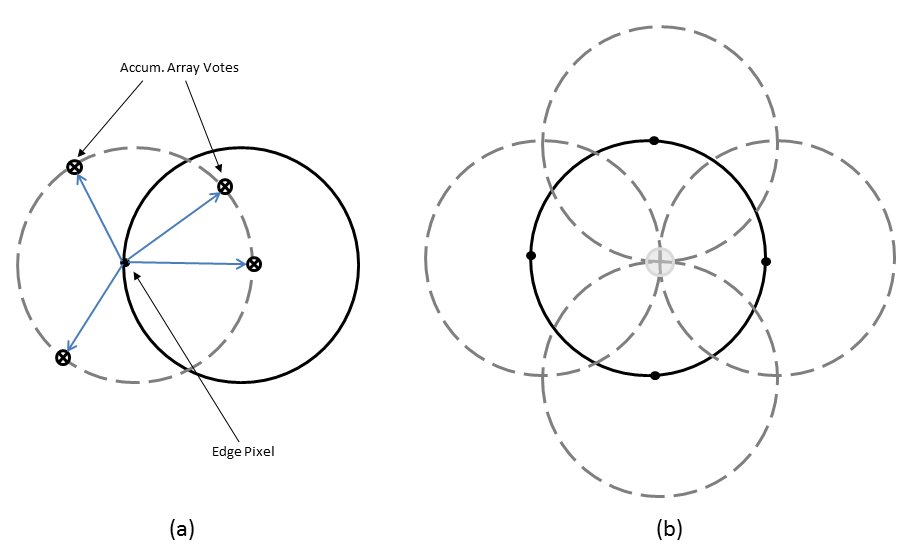
\includegraphics[scale=0.4]{img/fd/accarray.png}
\caption{CHT voting pattern to estimate the center of the circle.}
\label{fig:CHT}
\end{figure}

The second step is to estimate a center point. The position votes from the candidate pixels belonging to an image circle, tend to accumulate at the center of the circle. Therefore, the center of the circle is estimated by detecting the peaks in the accumulator array.


